%----------------------------------------------------------------------------------------
%	PACKAGES AND OTHER DOCUMENT CONFIGURATIONS
%----------------------------------------------------------------------------------------

\documentclass[11pt,fleqn]{book} % Default font size and left-justified equations

\usepackage[top=3cm,bottom=3cm,left=3.2cm,right=3.2cm,headsep=10pt,letterpaper]{geometry} % Page margins
\usepackage{xcolor} % Required for specifying colors by name
\definecolor{ocre}{RGB}{52,177,201} % Define the orange color used for highlighting throughout the book
\usepackage[section]{placeins}
% Font Settings
%\usepackage{avant} % Use the Avantgarde font for headings
%\usepackage{times} % Use the Times font for headings
%\usepackage{mathptmx} % Use the Adobe Times Roman as the default text font together with math symbols from the Sym­bol, Chancery and Com­pr Modern fonts

\usepackage{microtype} % Slightly tweak font spacing for aesthetics
\usepackage[utf8]{inputenc} % Required for including letters with accents
\usepackage[T1]{fontenc} % Use 8-bit encoding that has 256 glyphs

\usepackage{textgreek}
\usepackage{caption}
\usepackage{subcaption}
\usepackage[fulldiodes,siunitx, nooldvoltagedirection]{circuitikz}
\usepackage{csquotes}
\usepackage{siunitx}

% Bibliography
\usepackage[
backend=biber,
style=alphabetic,
sorting=ynt
]{biblatex}
\addbibresource{bibliography.bib}

\usepackage{makeidx}\makeindex 
%%%%%%%%%%%%%%%%%%%%%%%%%%%%%%%%%%%%%%%%%
% This is based on the Legrand Orange Book
% Structural Definitions File
%
% The original template (the Legrand Orange Book Template) can be found here --> http://www.latextemplates.com/template/the-legrand-orange-book
%
% Original author of the Legrand Orange Book Template::
% Mathias Legrand (legrand.mathias@gmail.com) with modifications by:
% Vel (vel@latextemplates.com)
%
% Original License:
% CC BY-NC-SA 3.0 (http://creativecommons.org/licenses/by-nc-sa/3.0/)
%
%%%%%%%%%%%%%%%%%%%%%%%%%%%%%%%%%%%%%%%%%
%----------------------------------------------------------------------------------------
%	VARIOUS REQUIRED PACKAGES
%----------------------------------------------------------------------------------------

\usepackage{titlesec} % Allows customization of titles

\usepackage{graphicx} % Required for including pictures
\graphicspath{{Pictures/}} % Specifies the directory where pictures are stored

\usepackage{lipsum} % Inserts dummy text

\usepackage{tikz} % Required for drawing custom shapes

\usepackage[english]{babel} % English language/hyphenation

\usepackage{enumitem} % Customize lists
\setlist{nolistsep} % Reduce spacing between bullet points and numbered lists

\usepackage{booktabs} % Required for nicer horizontal rules in tables

\usepackage{eso-pic} % Required for specifying an image background in the title page

%----------------------------------------------------------------------------------------
%	MAIN TABLE OF CONTENTS
%----------------------------------------------------------------------------------------

\usepackage{titletoc} % Required for manipulating the table of contents

\contentsmargin{0cm} % Removes the default margin
% Chapter text styling
\titlecontents{chapter}[1.25cm] % Indentation
{\addvspace{15pt}\large\sffamily\bfseries} % Spacing and font options for chapters
{\color{ocre!60}\contentslabel[\Large\thecontentslabel]{1.25cm}\color{ocre}} % Chapter number
{}  
{\color{ocre!60}\normalsize\sffamily\bfseries\;\titlerule*[.5pc]{.}\;\thecontentspage} % Page number
% Section text styling
\titlecontents{section}[1.25cm] % Indentation
{\addvspace{5pt}\sffamily\bfseries} % Spacing and font options for sections
{\contentslabel[\thecontentslabel]{1.25cm}} % Section number
{}
{\sffamily\hfill\color{black}\thecontentspage} % Page number
[]
% Subsection text styling
\titlecontents{subsection}[1.25cm] % Indentation
{\addvspace{1pt}\sffamily\small} % Spacing and font options for subsections
{\contentslabel[\thecontentslabel]{1.25cm}} % Subsection number
{}
{\sffamily\;\titlerule*[.5pc]{.}\;\thecontentspage} % Page number
[] 

%----------------------------------------------------------------------------------------
%	MINI TABLE OF CONTENTS IN CHAPTER HEADS
%----------------------------------------------------------------------------------------

% Section text styling
\titlecontents{lsection}[0em] % Indendating
{\footnotesize\sffamily} % Font settings
{}
{}
{}

% Subsection text styling
\titlecontents{lsubsection}[.5em] % Indentation
{\normalfont\footnotesize\sffamily} % Font settings
{}
{}
{}
 
%----------------------------------------------------------------------------------------
%	PAGE HEADERS
%----------------------------------------------------------------------------------------

\usepackage{fancyhdr} % Required for header and footer configuration

\pagestyle{fancy}
\renewcommand{\chaptermark}[1]{\markboth{\sffamily\normalsize\bfseries\chaptername\ \thechapter.\ #1}{}} % Chapter text font settings
\renewcommand{\sectionmark}[1]{\markright{\sffamily\normalsize\thesection\hspace{5pt}#1}{}} % Section text font settings
\fancyhf{} \fancyhead[LE,RO]{\sffamily\normalsize\thepage} % Font setting for the page number in the header
\fancyhead[LO]{\rightmark} % Print the nearest section name on the left side of odd pages
\fancyhead[RE]{\leftmark} % Print the current chapter name on the right side of even pages
\renewcommand{\headrulewidth}{0.5pt} % Width of the rule under the header
\addtolength{\headheight}{2.5pt} % Increase the spacing around the header slightly
\renewcommand{\footrulewidth}{0pt} % Removes the rule in the footer
\fancypagestyle{plain}{\fancyhead{}\renewcommand{\headrulewidth}{0pt}} % Style for when a plain pagestyle is specified

% Removes the header from odd empty pages at the end of chapters
\makeatletter
\renewcommand{\cleardoublepage}{
\clearpage\ifodd\c@page\else
\hbox{}
\vspace*{\fill}
\thispagestyle{empty}
\newpage
\fi}

%----------------------------------------------------------------------------------------
%	THEOREM STYLES
%----------------------------------------------------------------------------------------

\usepackage{amsmath,amsfonts,amssymb,amsthm} % For math equations, theorems, symbols, etc
\let\Bbbk\relax
\usepackage{txfonts}
\newcommand{\intoo}[2]{\mathopen{]}#1\,;#2\mathclose{[}}
\newcommand{\ud}{\mathop{\mathrm{{}d}}\mathopen{}}
\newcommand{\intff}[2]{\mathopen{[}#1\,;#2\mathclose{]}}
\newtheorem{notation}{Notation}[chapter]

%%%%%%%%%%%%%%%%%%%%%%%%%%%%%%%%%%%%%%%%%%%%%%%%%%%%%%%%%%%%%%%%%%%%%%%%%%%
%%%%%%%%%%%%%%%%%%%% dedicated to boxed/framed environements %%%%%%%%%%%%%%
%%%%%%%%%%%%%%%%%%%%%%%%%%%%%%%%%%%%%%%%%%%%%%%%%%%%%%%%%%%%%%%%%%%%%%%%%%%
\newtheoremstyle{ocrenumbox}% % Theorem style name
{0pt}% Space above
{0pt}% Space below
{\normalfont}% % Body font
{}% Indent amount
{\small\bf\sffamily\color{ocre}}% % Theorem head font
{\;}% Punctuation after theorem head
{0.25em}% Space after theorem head
{\small\sffamily\color{ocre}\thmname{#1}\nobreakspace\thmnumber{\@ifnotempty{#1}{}\@upn{#2}}% Theorem text (e.g. Theorem 2.1)
\thmnote{\nobreakspace\the\thm@notefont\sffamily\bfseries\color{black}---\nobreakspace#3.}} % Optional theorem note
\renewcommand{\qedsymbol}{$\blacksquare$}% Optional qed square

\newtheoremstyle{blacknumex}% Theorem style name
{5pt}% Space above
{5pt}% Space below
{\normalfont}% Body font
{} % Indent amount
{\small\bf\sffamily}% Theorem head font
{\;}% Punctuation after theorem head
{0.25em}% Space after theorem head
{\small\sffamily{\tiny\ensuremath{\blacksquare}}\nobreakspace\thmname{#1}\nobreakspace\thmnumber{\@ifnotempty{#1}{}\@upn{#2}}% Theorem text (e.g. Theorem 2.1)
\thmnote{\nobreakspace\the\thm@notefont\sffamily\bfseries---\nobreakspace#3.}}% Optional theorem note

\newtheoremstyle{blacknumbox} % Theorem style name
{0pt}% Space above
{0pt}% Space below
{\normalfont}% Body font
{}% Indent amount
{\small\bf\sffamily}% Theorem head font
{\;}% Punctuation after theorem head
{0.25em}% Space after theorem head
{\small\sffamily\thmname{#1}\nobreakspace\thmnumber{\@ifnotempty{#1}{}\@upn{#2}}% Theorem text (e.g. Theorem 2.1)
\thmnote{\nobreakspace\the\thm@notefont\sffamily\bfseries---\nobreakspace#3.}}% Optional theorem note

%%%%%%%%%%%%%%%%%%%%%%%%%%%%%%%%%%%%%%%%%%%%%%%%%%%%%%%%%%%%%%%%%%%%%%%%%%%
%%%%%%%%%%%%% dedicated to non-boxed/non-framed environements %%%%%%%%%%%%%
%%%%%%%%%%%%%%%%%%%%%%%%%%%%%%%%%%%%%%%%%%%%%%%%%%%%%%%%%%%%%%%%%%%%%%%%%%%
\newtheoremstyle{ocrenum}% % Theorem style name
{5pt}% Space above
{5pt}% Space below
{\normalfont}% % Body font
{}% Indent amount
{\small\bf\sffamily\color{ocre}}% % Theorem head font
{\;}% Punctuation after theorem head
{0.25em}% Space after theorem head
{\small\sffamily\color{ocre}\thmname{#1}\nobreakspace\thmnumber{\@ifnotempty{#1}{}\@upn{#2}}% Theorem text (e.g. Theorem 2.1)
\thmnote{\nobreakspace\the\thm@notefont\sffamily\bfseries\color{black}---\nobreakspace#3.}} % Optional theorem note
\renewcommand{\qedsymbol}{$\blacksquare$}% Optional qed square
\makeatother

% Defines the theorem text style for each type of theorem to one of the three styles above
\newcounter{dummy} 
\numberwithin{dummy}{section}
\theoremstyle{ocrenumbox}
\newtheorem{theoremeT}[dummy]{Theorem}
\newtheorem{problem}{Problem}[chapter]
\newtheorem{exerciseT}{Exercise}[chapter]
\theoremstyle{blacknumex}
\newtheorem{exampleT}{Example}[chapter]
\theoremstyle{blacknumbox}
\newtheorem{vocabulary}{Vocabulary}[chapter]
\newtheorem{definitionT}{Definition}[section]
\newtheorem{corollaryT}[dummy]{Corollary}
\theoremstyle{ocrenum}
\newtheorem{proposition}[dummy]{Proposition}

%----------------------------------------------------------------------------------------
%	DEFINITION OF COLORED BOXES
%----------------------------------------------------------------------------------------

\RequirePackage[framemethod=default]{mdframed} % Required for creating the theorem, definition, exercise and corollary boxes

% Theorem box
\newmdenv[skipabove=7pt,
skipbelow=7pt,
backgroundcolor=black!5,
linecolor=ocre,
innerleftmargin=5pt,
innerrightmargin=5pt,
innertopmargin=5pt,
leftmargin=0cm,
rightmargin=0cm,
innerbottommargin=5pt]{tBox}

% Exercise box	  
\newmdenv[skipabove=7pt,
skipbelow=7pt,
rightline=false,
leftline=true,
topline=false,
bottomline=false,
backgroundcolor=ocre!10,
linecolor=ocre,
innerleftmargin=5pt,
innerrightmargin=5pt,
innertopmargin=5pt,
innerbottommargin=5pt,
leftmargin=0cm,
rightmargin=0cm,
linewidth=4pt]{eBox}	

% Definition box
\newmdenv[skipabove=7pt,
skipbelow=7pt,
rightline=false,
leftline=true,
topline=false,
bottomline=false,
linecolor=ocre,
innerleftmargin=5pt,
innerrightmargin=5pt,
innertopmargin=0pt,
leftmargin=0cm,
rightmargin=0cm,
linewidth=4pt,
innerbottommargin=0pt]{dBox}	

% Corollary box
\newmdenv[skipabove=7pt,
skipbelow=7pt,
rightline=false,
leftline=true,
topline=false,
bottomline=false,
linecolor=gray,
backgroundcolor=black!5,
innerleftmargin=5pt,
innerrightmargin=5pt,
innertopmargin=5pt,
leftmargin=0cm,
rightmargin=0cm,
linewidth=4pt,
innerbottommargin=5pt]{cBox}

% Creates an environment for each type of theorem and assigns it a theorem text style from the "Theorem Styles" section above and a colored box from above
\newenvironment{theorem}{\begin{tBox}\begin{theoremeT}}{\end{theoremeT}\end{tBox}}
\newenvironment{exercise}{\begin{eBox}\begin{exerciseT}}{\hfill{\color{ocre}\tiny\ensuremath{\blacksquare}}\end{exerciseT}\end{eBox}}				  
\newenvironment{definition}{\begin{dBox}\begin{definitionT}}{\end{definitionT}\end{dBox}}	
\newenvironment{example}{\begin{exampleT}}{\hfill{\tiny\ensuremath{\blacksquare}}\end{exampleT}}		
\newenvironment{corollary}{\begin{cBox}\begin{corollaryT}}{\end{corollaryT}\end{cBox}}	

%----------------------------------------------------------------------------------------
%	REMARK ENVIRONMENT
%----------------------------------------------------------------------------------------

\newenvironment{remark}{\par\vspace{10pt}\small % Vertical white space above the remark and smaller font size
\begin{list}{}{
\leftmargin=35pt % Indentation on the left
\rightmargin=25pt}\item\ignorespaces % Indentation on the right
\makebox[-2.5pt]{\begin{tikzpicture}[overlay]
\node[draw=ocre!60,line width=1pt,circle,fill=ocre!25,font=\sffamily\bfseries,inner sep=2pt,outer sep=0pt] at (-15pt,0pt){\textcolor{ocre}{R}};\end{tikzpicture}} % Orange R in a circle
\advance\baselineskip -1pt}{\end{list}\vskip5pt} % Tighter line spacing and white space after remark

%----------------------------------------------------------------------------------------
%	SECTION NUMBERING IN THE MARGIN
%----------------------------------------------------------------------------------------

\makeatletter
\renewcommand{\@seccntformat}[1]{\llap{\textcolor{ocre}{\csname the#1\endcsname}\hspace{1em}}}                    
\renewcommand{\section}{\@startsection{section}{1}{\z@}
{-4ex \@plus -1ex \@minus -.4ex}
{1ex \@plus.2ex }
{\normalfont\large\sffamily\bfseries}}
\renewcommand{\subsection}{\@startsection {subsection}{2}{\z@}
{-3ex \@plus -0.1ex \@minus -.4ex}
{0.5ex \@plus.2ex }
{\normalfont\sffamily\bfseries}}
\renewcommand{\subsubsection}{\@startsection {subsubsection}{3}{\z@}
{-2ex \@plus -0.1ex \@minus -.2ex}
{.2ex \@plus.2ex }
{\normalfont\small\sffamily\bfseries}}                        
\renewcommand\paragraph{\@startsection{paragraph}{4}{\z@}
{-2ex \@plus-.2ex \@minus .2ex}
{.1ex}
{\normalfont\small\sffamily\bfseries}}

%----------------------------------------------------------------------------------------
%	HYPERLINKS IN THE DOCUMENTS
%----------------------------------------------------------------------------------------

% For an unclear reason, the package should be loaded now and not later
\usepackage{hyperref}
\hypersetup{hidelinks,colorlinks=false,breaklinks=true,urlcolor= ocre,pdftitle={Title},pdfauthor={Author}}
%backref=true,pagebackref=true,hyperindex=true,bookmarksopen=false,bookmarks=true
%----------------------------------------------------------------------------------------
%	CHAPTER HEADINGS
%----------------------------------------------------------------------------------------

% The set-up below should be (sadly) manually adapted to the overall margin page septup controlled by the geometry package loaded in the main.tex document. It is possible to implement below the dimensions used in the goemetry package (top,bottom,left,right)... TO BE DONE

\newcommand{\thechapterimage}{}
\newcommand{\chapterimage}[1]{\renewcommand{\thechapterimage}{#1}}

% Numbered chapters with mini tableofcontents
\def\thechapter{\arabic{chapter}}
\def\@makechapterhead#1{
\thispagestyle{empty}
{\centering \normalfont\sffamily
\ifnum \c@secnumdepth >\m@ne
\if@mainmatter
\startcontents
\begin{tikzpicture}[remember picture,overlay]
\node at (current page.north west)
{\begin{tikzpicture}[remember picture,overlay]
\node[anchor=north west,inner sep=0pt] at (0,0) {\includegraphics[width=\paperwidth]{\thechapterimage}};
%%%%%%%%%%%%%%%%%%%%%%%%%%%%%%%%%%%%%%%%%%%%%%%%%%%%%%%%%%%%%%%%%%%%%%%%%%%%%%%%%%%%%
% Commenting the 3 lines below removes the small contents box in the chapter heading
%\fill[color=ocre!10!white,opacity=.6] (1cm,0) rectangle (8cm,-7cm);
%\node[anchor=north west] at (1.1cm,.35cm) {\parbox[t][8cm][t]{6.5cm}{\huge\bfseries\flushleft \printcontents{l}{1}{\setcounter{tocdepth}{2}}}};
\draw[anchor=west] (8cm,-7cm) node []{\Huge\sffamily\bfseries\textcolor{black}{\thechapter. #1\strut\makebox[20cm]{}}};
%%%%%%%%%%%%%%%%%%%%%%%%%%%%%%%%%%%%%%%%%%%%%%%%%%%%%%%%%%%%%%%%%%%%%%%%%%%%%%%%%%%%%
\end{tikzpicture}};
\end{tikzpicture}}
\par\vspace*{230\p@}
\fi
\fi}

% Unnumbered chapters without mini tableofcontents (could be added though) 
\def\@makeschapterhead#1{
\thispagestyle{empty}
{\centering \normalfont\sffamily
\ifnum \c@secnumdepth >\m@ne
\if@mainmatter
\begin{tikzpicture}[remember picture,overlay]
\node at (current page.north west)
{\begin{tikzpicture}[remember picture,overlay]
\node[anchor=north west,inner sep=0pt] at (0,0) {\includegraphics[width=\paperwidth]{\thechapterimage}};
\draw[anchor=west] (8cm,-7cm) node []{\huge\sffamily\bfseries\textcolor{black}{#1\strut\makebox[22cm]{}}};
\end{tikzpicture}};
\end{tikzpicture}}
\par\vspace*{230\p@}
\fi
\fi
}
\makeatother % Insert the commands.tex file which contains the majority of the structure behind the template

\begin{document}
\title{Electromagnetism Explorer Kit}

%----------------------------------------------------------------------------------------
%	TITLE PAGE
%----------------------------------------------------------------------------------------

\begingroup
\thispagestyle{empty}
\AddToShipoutPicture*{\put(0,0){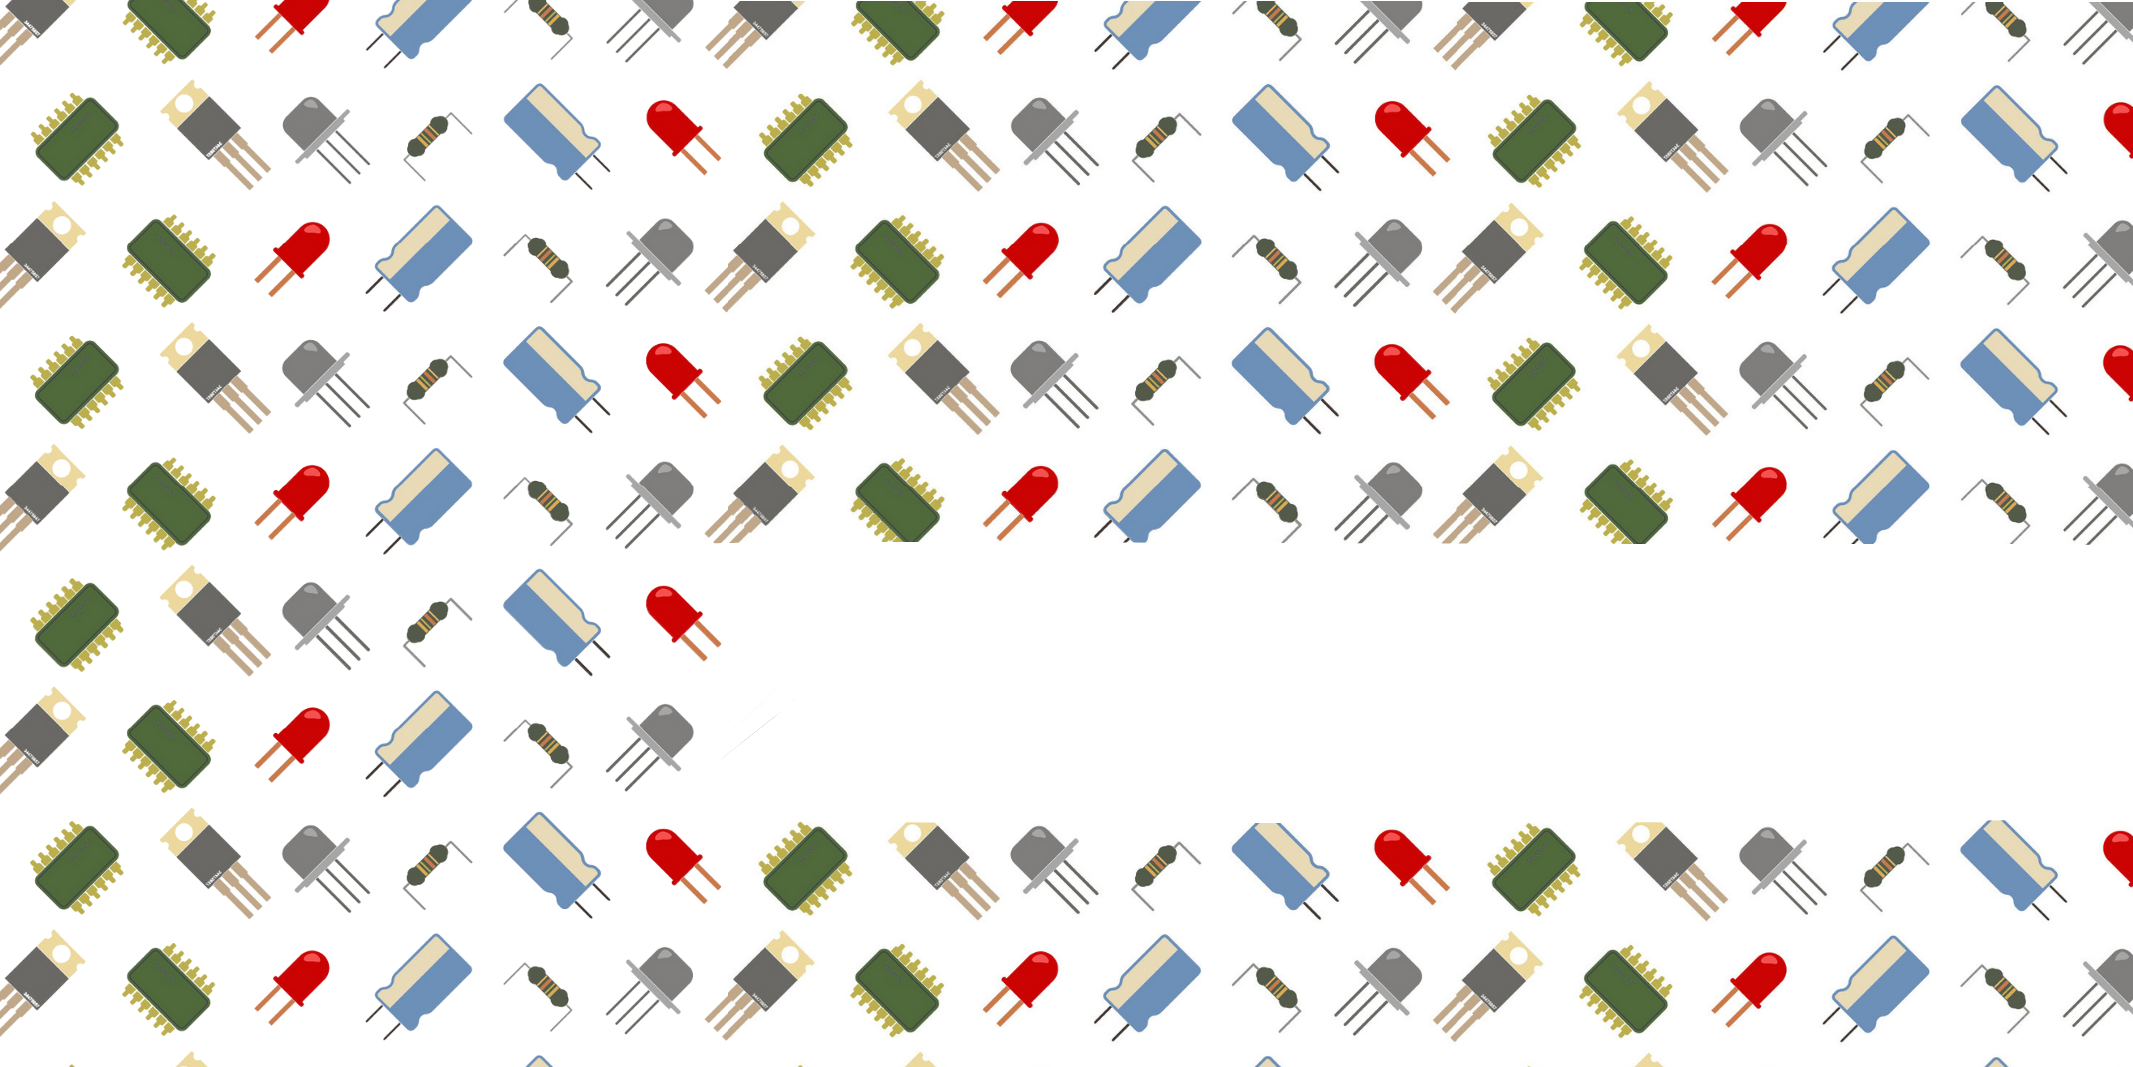
\includegraphics[width=\paperwidth]{chap_head.png}}} % Image background
\centering
\vspace*{5cm}
\par\normalfont\fontsize{35}{35}\sffamily\selectfont
%\textbf{Electronics Starter Kit}\\
%{\LARGE Learn | Experiment | Fun}\par % Book title
\vspace*{1cm}
%{\Huge HatchnHack}\par % Author name
\endgroup

%----------------------------------------------------------------------------------------
%	COPYRIGHT PAGE
%----------------------------------------------------------------------------------------

\newpage
~\vfill
\thispagestyle{empty}

%\noindent Copyright \copyright\ 2014 Andrea Hidalgo\\ % Copyright notice

\noindent \textsc{HatchnHack - A nest to your ideas}\\

\noindent \textsc{https://github.com/hatchnhack/Electronics-Starter-Kit}\\ % URL

\noindent \textit{First release, September 2020} % Printing/edition date

%----------------------------------------------------------------------------------------
%	TABLE OF CONTENTS
%----------------------------------------------------------------------------------------

\chapterimage{chap_head.png} % Table of contents heading image

\pagestyle{empty} % No headers

\tableofcontents % Print the table of contents itself

%\cleardoublepage % Forces the first chapter to start on an odd page so it's on the right

\pagestyle{fancy} % Print headers again
%----------------------------------------------------------------------------------------
%	CHAPTER 1
%----------------------------------------------------------------------------------------
\cleardoublepage
\chapterimage{chap_head.png} % Chapter heading image

\chapter{Homopolar Motor}
A motor is, elementarily, a device which converts electrical energy into
mechanical energy and kids know it as something which moves or rotates.
But one may question as to how exactly do these motors produce the rotational
force. This rotational force is due to the interaction between an electric current
and a magnetic field oriented in a specific direction. This basic principle can
be seen in action and appreciated better with a simple demonstration of a
homopolar motor. The homopolar motor, first created in 1821 by Michael
Faraday, is the most fundamental example of a motor, and is really fun to
experiment with.

\section{What all you need}
\begin{itemize}
    \item Duracell AA Battery(1.5V)
    \item Tapered Screw
    \item Insulated Copper Wire
    \item Neodymium Magnet (diameter - 12mm)
    \item A piece of paper (optional)
\end{itemize}

\section{Get ready to build the world’s simplest motor}
There is no better way to learn how a motor works than by building your very
own motor! Here is what you have to do:
\begin{itemize}
    \item[Step 1:] Attach the head of the screw to the magnet as shown in Fig
    \item[Step 2:] Connect the pointed side of the screw to the negative terminal of the battery as shown in Fig 
    \item[Step 3:] Use the insulated copper wire to connect the positive terminal of the battery to the side of the 
        magnet. Be careful that the wire should touch the side of the magnet at right angles and not at its bottom. 
\end{itemize}

\section{Understanding the principle behind}
When the screw is connected to the magnet, it gets magnetized. As soon as the wire is connected from one end of the 
battery to the side of the magnet (and not the bottom), the circuit gets completed. The rotation is produced because 
the direction of current and that of the magnetic field is perpendicular to each other. In this case, a force (known 
as Lorentz Force) is exerted in a direction perpendicular to BOTH of them, causing the spinning motion. Fig 2.5 specifies 
the directions of the Current, magnetic field and force. The direction is given by Fleming’s Left Hand Rule (shown in 
Fig 2.6); which says that if the thumb, forefinger and middle finger of the left hand are stretched to be perpendicular 
to each other, and if the fore finger represents the direction of magnetic field, the middle finger represents the 
direction of current, then the thumb represents the direction of force.

The following mathematical equation represents the relationship:
\begin{equation*}
    F = I(\overrightarrow{L} \times \overrightarrow{B})
\end{equation*}
The stronger the magnet, the faster the wire will rotate. Neodymium magnets are the strongest in the world and therefore, 
while using an AA battery to make a homopolar motor, an ideal magnet to use is a 12mm diameter and a 6mm thick neodymium magnet.

\section{Thinking Beyond}
Now, you know how the simplest motor works and it is, in fact, true for all of the DC motors that you can think of. From 
the industrial fans, household devices like the food processor, food mixers, electric watches to the largest instances in 
automotive and ship propulsion, this principle is followed. Generally, an electric motor would contain a coil of wire that 
can create an electromagnetic field aligned with the centre of the coil, when electricity flows through it. This wire is 
referred to as an electromagnet. The magnetic field may be created using permanent magnets as well. When, a current is sent 
through this loop of wire, the electromagnet experiences a Lorentz force on it at right angles to the direction of the 
magnetic field and the current flowing. And this force causes the loop of wire to generate mechanical energy and rotate.

Why is this motor called homopolar motor? The homopolar motor gets its name from the fact that the direction of the electrical
current and the magnetic field never reverses, unlike an AC motor, or a DC motor containing a commutator.

What more can you do? One may add a paper fan as shown in Fig 2.7 to this homopolar motor to see the motor actually rotating, 
even from a far distance. Just by adding a piece of paper or some plastic blades between the screw head and the magnet, you 
can see that as the screw rotates, the blades/paper rotates!

You can even bend a wire to form any shape, for example, a wired Ballerina! The shape of the wire should be such that allows 
it to balance properly, otherwise it might fall off the battery when it begins to spin.
%----------------------------------------------------------------------------------------
%	CHAPTER 2
%----------------------------------------------------------------------------------------
\cleardoublepage
\chapterimage{chap_head.png} % Chapter heading image

\chapter{Faraday Generator}
Science is taught to us through textbooks. But not only can we observe
various physical laws in real, we can also apply them to make cool stuff
that demonstrates them. For example, conversion of one form of energy to
another is a fascinating event to see. The glowing LED faraday generator is a
perfect demonstration of Faraday’s law. The fundamental principles behind
the generation of electricity were based on Michael Faraday’s discoveries in
the nineteenth century. This DIY kinetic generator converts your mechanical
power (just a number of shakes) to electrical power, based on his principle.

\section{What all you need}
To make your own glowing LED Faraday Generator, you will need the
following materials:
\begin{itemize}
    \item Thread spool $\times$ 1
    \item Enameled copper wire: 36-SWG $\times$ 50m
    \item Red LEDs $\times$ 2
    \item Neodymium Magnet (diameter- 7 mm) $\times$ 1
    \item Matchsticks $\times$ 2
    \item Needle/Compass $\times$ 1
    \item Sand Paper
    \item Watchmaker’s File $\times$ 1
    \item Insulation Tape
    \item Soldering Equipment*
\end{itemize}

\section{Understanding the principle behind}
Before we apply the science, we must know the science. Michael Faraday, a
master experimentalist of the nineteenth century, is best known for his invention of the phenomena of electromagnetic induction and that of the electric
generator and motor. This was, in fact, his most revered contribution to two
of the most coveted and bewildering subjects of science and innovation at
that time, Electricity and Magnetism. His work formed a strong basis for the
merger of these two, and its significance is paramount. The invention of an
electric generator and motor finds application in almost every appliance today.
From washing machines to fans, to food mixers and electric chargers, all use
Faraday’s theory of electromagnetic induction. The glowing LED faraday
generator works on the Faraday’s law of electromagnetic induction which
states that:

\textbf{\emph{“The induced electromotive force (or voltage) in any closed circuit is
equal to the negative of the time rate of change of the magnetic flux
enclosed by the circuit.”}}

Here, your closed circuit is going to be the 50 m of copper wire wound
around the thread spool and the magnetic flux is changed by shaking the
thread spool. This changes the magnetic field due to the up-down motion of
the magnet. The change of magnetic field as seen by the wire, generates an
electromagnetic force(EMF) that is proportional to the number of turns of
wire, as well as the rate at which the magnetic field is changed.

\section{Get Ready to Shake and Generate}
To make your own LED glowing faraday generator, all you need to do is to
follow a set of few simple steps:

\begin{itemize}
    \item[Step 1:] Start by creating two marks on the thread spool, with the help of pen
        or a marker, such that the distance between them is equal to the length
        of the magnet.
    \item[Step 2:] Now, with the help of a needle, pierce the thread spool at these marks
        as shown in Fig 3.2 such that you have holes on both the sides of the
        thread spool. Be careful, it would hurt if the needle pierces your finger
        instead of the thread spool.
    \item[Step 3:] Using a watchmaker’s file, file those holes and inside of the thread
        spool for smooth movement of the magnet inside the spool. Also, make
        sure that the holes are big enough to put a matchstick in them. Once
        the filing is done, put two matchsticks in these holes as shown in Fig
        3.3.
    \item[Step 4:] Now, we start winding the copper wire. Leave 6 to 8 cm of wire, wind
        5-6 turns on one of the matchsticks and then start winding on the thread
        spool. By doing this, we fix one end of the wire. Be careful that you
        wind the copper wire between the matchsticks only. Have patience, it
        will take some time.
    \item[Step 5:] Once the winding is done, put tape around the windings and then
        remove the matchsticks. Be careful not to stick ends of the wire inside
        the tape. 
    \item[Step 6:] Since we are using ‘enameled’ copper wire, we need to remove the
        enamel at the ends of the wire to make the connections. Sand the ends
        using a sandpaper very slowly and lightly, or otherwise, the wire might
        break.
    \item[Step 7:] Now is the time for soldering. Solder two LEDs at the ends of the
        wire in opposite polarities (You can identify the polarity of an LED by
        seeing the length of its legs, the longer one is positive and the shorter
        one is negative). 
\end{itemize}
\textbf{NOTE:} 

The reason for opposite polarity of LEDs is Lenz’s law which states
that:

\textbf{\emph{“The direction of current induced in a conductor by a changing
magnetic field due to Faraday’s law of induction will be such that
it will create a magnetic field that opposes the change that produced it.”}}

Hence, if a clockwise current is induced due to the upward motion of
the magnet, then an anti-clockwise current will be induced due to the
downward motion of the magnet. Thus, if one LED glows when the
magnet goes up, the other will glow when the magnet goes down.
\begin{itemize}[resume]
    \item[Step 8:] Now stick the LEDs on the thread spool using tape. Stick them 180
        degrees apart so that you can see both of them glowing separately. And
        you are done! Your glowing LED Faraday Generator is ready. Insert
        your magnet inside the spool and as you move the thread spool updown, you can see the LEDs glowing.    
\end{itemize}

\section{Thinking Beyond}
This Faraday Generator, when shaken vigorously, can be used to generate
sufficient energy to charge up capacitors. This energy stored in capacitors
can be utilized in powering low power circuits. How about your TV Remote?
You can get rid of those batteries with a Kinetic Remote or an Electronic Dice
which gives a random number when you shake it!
%----------------------------------------------------------------------------------------
%	CHAPTER 3
%----------------------------------------------------------------------------------------
\cleardoublepage
\chapterimage{chap_head.png} % Chapter heading image

\chapter{DC Motor}
A DC motor is a device which converts electrical energy into mechanical
energy. One may find DC motors in many portable home appliances like
fans, food mixers, in automobiles and in numerous industrial equipment. The
rotational force is due to the interaction between an electric current and a
magnetic field, both of which are oriented in specific different directions.
This manual will help you make a very impressive motor of your own!

\section{What all you need}
\begin{itemize}
    \item Zero PCB
    \item Hook up wires
    \item Insulated copper wires (single strand)
    \item Enameled copper wire(21 SWG)
    \item Neodymium magnets (diameter -12mm)
    \item Wire cutter
    \item Sand paper
    \item Double sided tape
    \item Duracell AA battery(1.5V)
    \item Paper Cutter
    \item Soldering Equipment
\end{itemize}

\section{Get Ready to make your own DC Motor!}
\begin{enumerate}
    \item[Step 1:] Creating the coil
        \begin{enumerate}
            \item Take the enameled copper wire (21 SWG) and cut a length of
                around 1 feet from it with the help of wire cutter as shown in Fig
                4.2.
            \item Take the AA battery and wrap the wire over the battery leaving approximately 2 inches of wire from each of the ends as shown
            in Fig 4.3.
            \item The coil should be tightly wound because a balanced coil will
            rotate more swiftly.
            \item Wrap the ends of the coil 2 or 3 times through the coil to make
            the coil maintain its shape.
            \item The trailing ends should be diametrically opposite to each other,
            for the symmetrical shape and for the balance of the motor.
        \end{enumerate} 
    \item[Step 2:] Removing the insulation from the ends of the coil 
        \item[] 
            The next step is a bit difficult and, so, has to be performed with care. The
            insulation of the ends of the coils has to be removed, to unleash the
            metal underneath it, to make it conducting. Take one end of the coil
            and start removing the enamel, using a paper cutter, leaving a shiny
            new layer of copper wire. The enamel from the end of the coil has to be
            removed from only one half of the perimeter of the wire, say, the upper
            half. Similarly, the insulation from the other end has to be removed
            from only the upper half of the perimeter. This process is done so that
            the force exerted by the magnet to the coil should be unidirectional,
            and the motion is sustained.The enamel should be removed properly to
            ensure a good electrical connection between the wire and coil. After
            this, you will have a coil that is ready to be the armature of your motor,
            as shown in Fig 4.6.
    \item[Step 3:] Creating posts for the motor coil to rotate
        \item[] The posts will form a stand for your motor, aiding its rotation.
        \begin{enumerate}
            \item To start building a stand for the motor, you need a Zero Board
            and two hookup wires.
            \item Measure the length of your coil end to end leaving 1 inch on
            either end and mark it on the Zero Board.
            \item Take a hookup wire of nearly 2 inches length and make it straight
            using a tweezer.
            \item Then make a small U-shape at one end of it through a plier/tweezer.
            \item Put it through the mark on the Zero Board from downwards side.
            Press the smaller end of the U-shaped post in the zero board, so
            that the wire stands straight. Repeat the process for the other wire
            as well.Now, you have two wire posts (each of lengths 2 inches)
            standing straight on the Zero Board. Solder the Hookup Wires in
            place.
            \item Using the plier, make a loop at the top end of each of the wires.
            Ensure that the loops are similar to both the posts.Now take your
            coil and try to suspend it with the help of these loops made on the
            posts.
            \item If it suspends in a perfectly horizontal fashion, then proceed.
            Otherwise, adjust the posts and the height of the loops to make it
            suspend horizontally.
        \end{enumerate}
    \item[Step 4:] Making the electrical connections
        \item[] For the electric current to flow through your coil, you need to connect
            the battery to the motor
        \begin{enumerate}
            \item Take two single strand copper wires, preferably 15 cm in length.
            \item Strip off its insulation up to half inches from either side, for both
            the wires.
            \item Take one wire and wrap one of its ends at the bottom end of a
            post, thus establishing a connection. Do the same with the other
            wire as well. Make sure that the connection should be strong
            enough to hold.            
        \end{enumerate}
    \item[Step 5:] Attaching the magnet
        \item[] Now it is time for assembling the most important part of this motor, the
            magnet.
        \begin{enumerate}
            \item Take the magnet and place it at the centre of the two posts and
            mark its place.
            \item Now cut a piece of double-sided tape and paste it at the mark
            you just made for the magnet. Take off the other covering of the
            tape at put the magnet there. Apply some pressure so that it holds
            good. Take care that the magnet should be around 2-3 cm below
            where the coil would be, and perfectly under it.        
        \end{enumerate}
    \item[Step 6:] Testing the motor and making the necessary twitches
        \begin{enumerate}
            \item Suspend the copper coil on the wire posts. Make sure that the
            exposed ends should make contact with the hookup wires.
            \item Take up the battery and fix one of one of the copper wires to the
            end of the wire through a tape, preferably, to fix a connection.
            Take the other end and complete the electrical circuit by touching
            it to the other end of the battery.
            \item The copper coil may start rotating on its own, but may also,
            sometimes, require a small push to start rotating. If the coil is not
            spinning after this, you may need to sand the ends of the coil or
            you may need to make the coil more balanced to make it rotate.
            Keep trying till it doesn’t start rotating!
        \end{enumerate} 
\end{enumerate}

\section{Understanding the principle behind}
A motor is an electrical machine which converts electrical energy into mechanical energy. The working principle behind in a motor is that, whenever
a current carrying conductor is placed in a magnetic field, it experiences
a force, according to the Fleming’s Left-Hand Rule (discussed on page 7).
When the armature coils are connected to a DC voltage supply, some current
starts flowing in the conductor. The magnetic field may be provided by electromagnets or by using permanent magnets. In this case, current carrying
armature conductors experience a force due to the magnetic field provided by
a neodymium magnet present near the base of the coil.

%----------------------------------------------------------------------------------------
%	BIBLIOGRAPHY
%----------------------------------------------------------------------------------------
\nocite{*}
\chapterimage{chap_head.png}
\addcontentsline{toc}{chapter}{\textcolor{ocre}{Bibliography}}
\printbibliography[title={References}]

\end{document}